\RequirePackage{fix-cm}
% Presentación para el advisor, en inglés: el terremoto, los mecanismos
% posibles, el diseño, el perfil de la salud mental por edad al terremoto en
% tramos de seis meses (el resultado principal), la misma comparación en
% tres rondas, el entorno socioeconómico y familiar, la lactancia y el
% estrés de la madre, y lo que queda abierto. La comparación resumen, los
% primeros 18 meses (6-17) frente a todas las demás edades, se eligió
% después de ver el perfil: es exploratoria.
% Figuras: python3 scripts/28_beamer_advisor.py
% Tablas: python3 scripts/41_tablas_apendice.py
% Compilar desde presentacion/: xelatex advisor.tex (dos veces)
\documentclass[aspectratio=169,11pt]{beamer}
\usepackage[english]{babel}
\usepackage{fontspec}
\usefonttheme{serif}
\newfontfamily\demi{Latin Modern Roman Demi}[Ligatures=TeX]
\usepackage{array}
\usepackage{booktabs}
\usepackage{pifont}
\usepackage{tikz}
\usepackage{appendixnumberbeamer}

\definecolor{ink}{HTML}{1A1A1A}
\definecolor{acc}{HTML}{1B6A4E}
\definecolor{muted}{HTML}{5C5C5C}
\definecolor{ocre}{HTML}{A06F00}
\definecolor{linea}{HTML}{CCCCCC}
\definecolor{azul}{HTML}{2B5FA8}

\setbeamercolor{normal text}{fg=ink,bg=white}
\setbeamercolor{frametitle}{fg=ink}
\setbeamercolor{structure}{fg=acc}
\setbeamerfont{frametitle}{size=\Large,family=\demi}
\setbeamertemplate{navigation symbols}{}
\setbeamertemplate{frametitle continuation}{}
\setbeamertemplate{frametitle}{\vspace*{5mm}\insertframetitle\par}
\setbeamertemplate{footline}{%
  \hfill{\scriptsize\color{muted}\insertframenumber\,/\,\inserttotalframenumber}%
  \hspace*{8mm}\vspace*{4mm}}
\setbeamersize{text margin left=8mm,text margin right=8mm}

\newcommand{\sub}[1]{{\leavevmode\color{muted}#1}}
\newcommand{\nota}[1]{\vfill\noindent\parbox{0.9\textwidth}{\scriptsize\color{muted}#1}\par\vspace*{1mm}}
\newcommand{\cita}[1]{{\footnotesize\color{azul}#1}}
\newcommand{\citanota}[1]{{\color{azul}#1}}
% revista de una referencia: enlace al DOI, en negrita y cursiva
\newcommand{\revista}[2]{\href{https://doi.org/#1}{{\bfseries\itshape #2}}}
\newcommand{\notachica}[1]{\vfill\noindent\parbox{\textwidth}{\fontsize{7}{8.4}\selectfont\color{muted}#1}\par\vspace*{1mm}}
\newcommand{\no}{{\leavevmode\color{ocre}\ding{55}}}
\newcommand{\si}{{\leavevmode\color{acc}\ding{51}}}
\newcommand{\canal}[2]{{\leavevmode\bfseries\color{#1}#2}}
% botones a las tablas del apéndice y de vuelta, en la esquina inferior izquierda
\setbeamercolor{button}{bg=acc!12,fg=acc}
\setbeamerfont{button}{size=\scriptsize}
\newcommand{\boton}[1]{\begin{tikzpicture}[remember picture,overlay]
  \node[anchor=south west,inner sep=0pt] at ([xshift=8mm,yshift=2.6mm]current page.south west) {#1};
  \end{tikzpicture}}
\newcommand{\tabla}[2]{\hyperlink{#1}{\beamergotobutton{#2}}}
\newcommand{\volver}[1]{\boton{\hyperlink{#1}{\beamerreturnbutton{Back}}}}

\title{The Timing of Early-Life Shocks and Adolescent Mental Health}
\date{October 2026}

\begin{document}

% ----------------------------------------------------------------- Título
\begin{frame}[plain,noframenumbering]
\vfill
\begin{center}
{\demi\LARGE The Timing of Early-Life Shocks\\[1.5mm] and Adolescent Mental Health\par}
\vspace{10mm}
{\small October 2026\par}
\end{center}
\vfill
\end{frame}

% ------------------------------------------------------------------ 1. Chile
\begin{frame}[label=chile]
\frametitle{Do the effects of an earthquake in early childhood persist?%
\boton{\tabla{figpga}{PGA map}}}
\begin{columns}[c,onlytextwidth]
\column{0.34\textwidth}
\centering
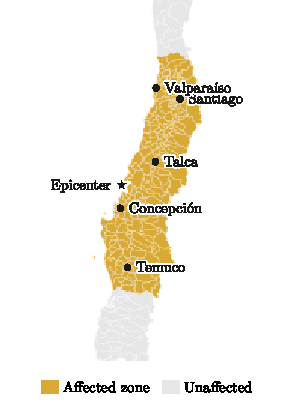
\includegraphics[height=0.74\textheight]{figuras/mapa.pdf}
\column{0.64\textwidth}
\renewcommand{\arraystretch}{1.45}
\begin{tabular}{@{}p{18mm}>{\raggedright\arraybackslash}p{70mm}@{}}
\textbf{Shock}   & 27 February 2010 (27-F), magnitude 8.8 \\
\textbf{Exposed} & Children aged 6 months to 4 years \\
\end{tabular}

\vspace{3mm}
{\small\bfseries Effects of early-childhood shocks\par}
\vspace{1.5mm}
{\small\raggedright
Birth weight \cita{(Torche, 2011)}\par\vspace{1mm}
Cognitive and non-cognitive development \cita{(Gillmore, 2026)}\par\vspace{1mm}
Height and learning \cita{(Andrabi, Daniels, and Das, 2023)}\par\vspace{1mm}
Adult mental health \cita{(Persson and Rossin-Slater, 2018)}\par}

\vspace{3mm}
{\small\bfseries This paper\par}
\vspace{1.5mm}
{\small\raggedright Mental health at ages 14--18 by age at the earthquake,\\ from 6 to 49 months\par
\vspace{0.6mm}{\footnotesize\color{muted}The 2024 round follows the 2010 cohort, born by August 2009:
exposure in utero or before 6 months is not observed\par}}
\end{columns}
\end{frame}

% ------------------------------------------------------------- 2. Pregunta
\begin{frame}
\vfill
\begin{center}
{\huge\bfseries Does it matter at what age\\[2mm] children live through the shock?\par}
\vspace{10mm}
\parbox{0.74\textwidth}{\large\hyphenpenalty=10000{\frenchspacing“The effects of stress on
the brain depend critically on the timing (age of onset and duration). When
stress occurs early in life it can have profound and lasting effects on brain
organization and function.”}
\mbox{\small\color{azul}(Gee and Casey, 2015, p.~184)}}\par
\end{center}
\vfill
\end{frame}

% ------------------------------------------------------------------ 3. Vías
\begin{frame}
\frametitle{Potential mechanisms}
\vspace{3mm}
{\small
\renewcommand{\arraystretch}{1.6}
\begin{tabular}{@{}>{\raggedright\arraybackslash}p{42mm}
                >{\raggedright\arraybackslash}p{96mm}@{}}
 & \sub{Channels} \\
\canal{ocre}{Socioeconomic and family environment}
 & The earthquake reduces income, damages housing, and increases conflict
   at home \cita{(Conger and Donnellan, 2007; Almond, Currie, and Duque,
   2018)} \\
\canal{ocre}{Transmission of\newline maternal stress}
 & Infants regulate their stress through the mother. If she is stressed, she
   passes it on through daily contact \cita{(Persson and Rossin-Slater, 2018)} \\
\end{tabular}}
\end{frame}

% ----------------------------------------------------------------- 3. Datos
\begin{frame}[label=datos]
\frametitle{Data\boton{\tabla{tabdesc}{Descriptives}}}
\vspace{3mm}
\centering
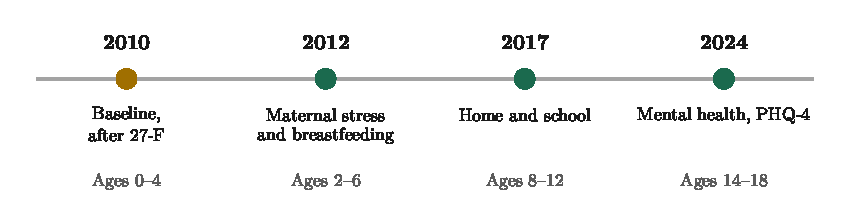
\includegraphics[width=\textwidth]{figuras/datos_elpi.pdf}

\vspace{3mm}
{\raggedright
\renewcommand{\arraystretch}{1.35}
\begin{tabular}{@{}>{\raggedright\arraybackslash}p{24mm}
                >{\raggedright\arraybackslash}p{108mm}@{}}
\sub{Survey}      & ELPI, Early Childhood Longitudinal Survey, Chile \\
\sub{Sample}      & 9,996 adolescents born between January 2006 and August 2009, aged 6 to 49 months on 27-F; 4,961 girls \\
\sub{Respondents} & The caregiver in every round; the child in 2017 and 2024 \\
\end{tabular}\par}
\end{frame}

% ----------------------------------------------------------------- 4. Diseño
\begin{frame}[label=spec]
\frametitle{Econometric specification%
\boton{\tabla{tabbal}{Balance}\hspace{1mm}\tabla{tabatr}{Attrition}}}
\vspace{0mm}
\begin{equation*}
Y_{imc} = \sum_{a} \beta_a\,(\mathrm{Age}_{ai} \times \mathrm{Affected}_m)
 + \sum_{a} \gamma_a\, \mathrm{Age}_{ai} + \psi_m + \theta_c + X_i'\delta + \varepsilon_{imc}
\end{equation*}
\vspace{-1mm}
{\small
\renewcommand{\arraystretch}{1.15}
\begin{tabular}{@{}l l@{}}
{\color{muted}$Y_{imc}$} & Mental health at ages 14--18, PHQ-4 \\
{\color{muted}$\mathrm{Age}_{ai}$} & Six-month age groups at the earthquake: 6--11, 12--17, \ldots, 42--49 months \\
{\color{muted}$\mathrm{Affected}_m$} & Municipality in the zone of destructive damage \\
{\color{muted}$\psi_m$, $\theta_c$} & Municipality and birth-year fixed effects \\
{\color{muted}$X_i$} & Linear trend in month of birth; child and household controls \\
\end{tabular}

\vspace{2mm}
\begin{tabular}{@{}>{\raggedright\arraybackslash}p{22mm}>{\raggedright\arraybackslash}p{116mm}@{}}
\textbf{Profile} & $\beta_a$ normalized to average zero; joint test of a flat profile \\
\textbf{Summary} & First 18 months relative to all other ages, chosen after inspecting the profile \\
\end{tabular}}

\nota{$\mathrm{Affected}_m$ does not vary within municipality, so $\psi_m$ absorbs the average
effect of the earthquake: the design identifies how the effect varies with age at exposure,
not its level. Replacing $\gamma_a$, $\theta_c$, and the trend with month-of-birth fixed
effects leaves the estimates unchanged.}
\end{frame}

% ----------------------------------------------------- 5. Perfil por edad
\begin{frame}[label=sm]
\frametitle{Age at exposure matters for girls, not for boys%
\boton{\tabla{figphq}{Distribution}\hspace{1mm}\tabla{figniv}{Levels}\hspace{1mm}%
\tabla{tabphq}{Table}\hspace{1mm}\tabla{tabgir}{Other outcomes}}}
\centering
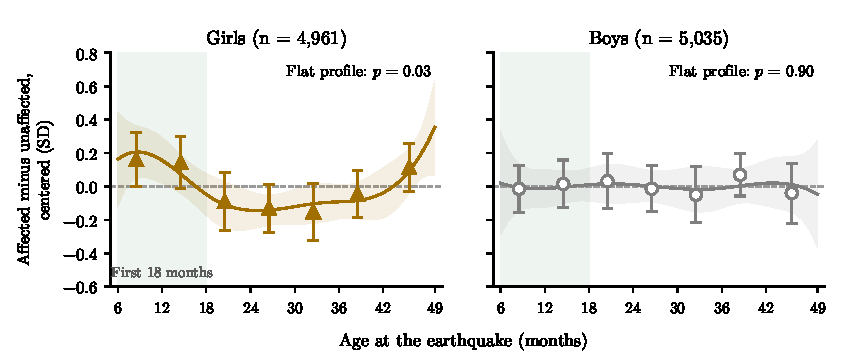
\includegraphics[width=0.84\textwidth]{figuras/perfil.pdf}

\nota{PHQ-4 \citanota{(Kroenke et al., 2009)}, four questions answered by the adolescent on
anxiety and depression. Affected minus unaffected in each six-month age group, normalized to
average zero; the curve is a B-spline in age in months; 95\% CI. Summary comparison, chosen
after inspecting the profile: the first 18 months relative to all other ages, 0.21 SD for girls
(SE 0.08; wild bootstrap $p = 0.01$; randomization across regions $p = 0.06$) and 0.00 for
boys; girls minus boys, 0.21 (SE 0.10).}
\end{frame}

% ------------------------------------------------------ 6. Tres rondas
\begin{frame}[label=olas]
\frametitle{Girls report the gap; their caregivers do not%
\boton{\tabla{tabola}{Table}\hspace{1mm}\tabla{figola}{Profiles}}}
\centering
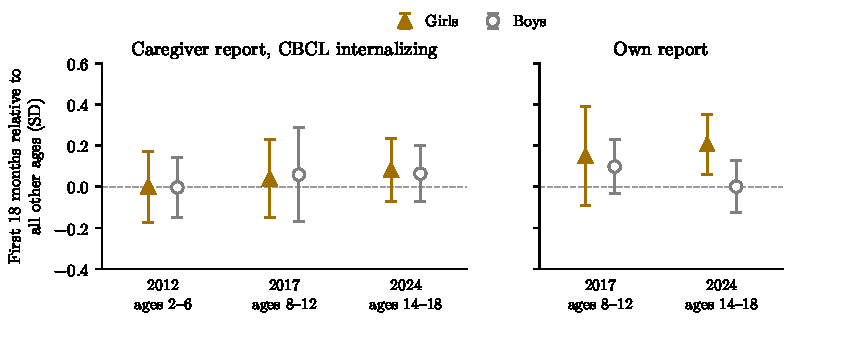
\includegraphics[width=0.84\textwidth]{figuras/tres_olas.pdf}

\nota{The same adolescents in each round, with the specification of the previous slide; 95\% CI.
Caregiver report, CBCL internalizing scale. Own report: in 2017, an index of low self-esteem,
not feeling happy, and feeling lonely in class; in 2024, the PHQ-4. Flat profile for girls:
$p = 0.03$ for the 2024 PHQ-4 and above 0.2 for the other four measures. Different
informants' reports of internalizing symptoms correlate at 0.25 on average \citanota{(De Los
Reyes et al., 2015)}.}
\end{frame}

% --------------------------------------------------------------- 7. Hogar
\begin{frame}[label=entorno]
\frametitle{Socioeconomic and family environment does not explain the gap%
\boton{\tabla{tabent}{Table}}}
{\small\raggedright The earthquake worsened the environment \cita{(Gillmore, 2026)},
but not more for those exposed in the first 18 months\par}
\centering
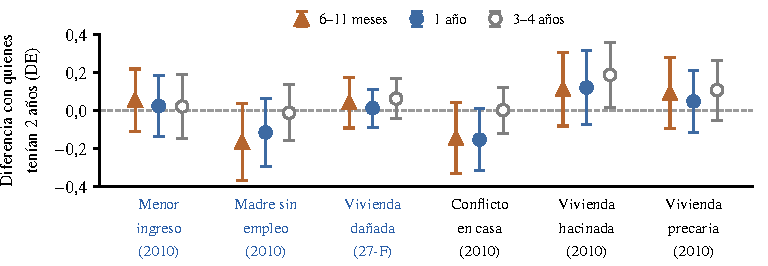
\includegraphics[scale=0.9]{figuras/canal_hogar.pdf}

\notachica{Measured in 2010, one to nine months after the earthquake, except housing
damage, reported in 2012. In blue, the mechanisms in \citanota{Gillmore (2026)}. Lower income, per capita; damaged housing,
destroyed or with major damage; conflict at home, the mother shouting, being
hostile, or hitting during the visit; overcrowded housing, persons per bedroom;
precarious housing, an emergency shack (\emph{mediagua}) or a lent or shared
dwelling. Girls exposed at 6--17 months relative to all other ages; 95\% CI. The two
estimates that differ from zero point to a better environment, not a worse one.}
\end{frame}

% ------------------------------------------------------------- 8. La madre
\begin{frame}[label=diada]
\frametitle{The effect is larger among breastfed girls, but imprecise%
\boton{\tabla{tablac}{Table}\hspace{1mm}\tabla{figlac}{By age}\hspace{1mm}%
\tabla{tabdia}{Maternal stress}\hspace{1mm}\tabla{tabmed}{Means}}}
\centering
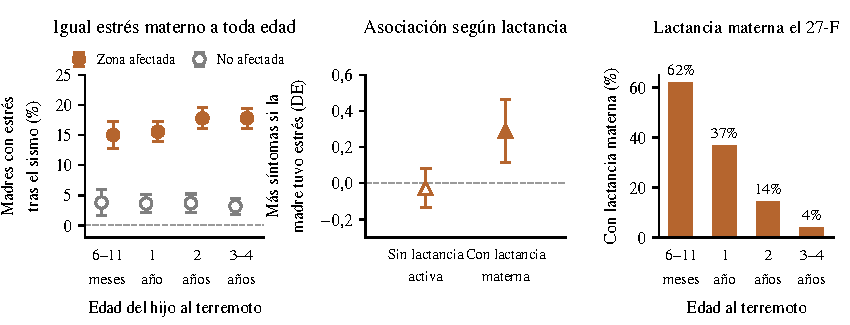
\includegraphics[width=0.92\textwidth]{figuras/diada.pdf}

\nota{Breastfed, still breastfed on 27-F (2012 report): 53\% of girls exposed at 6--17
months. Left, with six-month age group $\times$ breastfed fixed effects; the difference
between breastfed and not breastfed is 0.23 SD (SE 0.17; wild bootstrap $p = 0.20$). Right,
the share of mothers who reported stress, distress, or anxiety after the earthquake, unweighted;
95\% CI. It did not rise more for the mothers of the youngest: for girls exposed at 6--17
months relative to all other ages, $-3.3$ points (SE 1.8).}
\end{frame}

% ------------------------------------------------------------ 9. Hallazgos
\begin{frame}
\frametitle{Findings}
\vspace{4mm}
\begin{itemize}\setlength{\itemsep}{4mm}
\item Among girls, the effect of the earthquake on mental health at ages 14--18 varies with
      age at exposure (flat profile rejected, $p = 0.03$); among boys, it does not ($p = 0.90$).
\item Girls exposed in the first 18 months report more symptoms than those exposed later,
      by 0.21 SD, a comparison chosen after inspecting the profile.
\item The gap is in the girls' own reports, significant in 2024 and of the same sign in 2017;
      their caregivers report no difference in 2012, 2017, or 2024.
\item The socioeconomic and family environment did not worsen more for the youngest, and
      the stress their mothers reported in 2012 did not rise more.
\end{itemize}
\end{frame}

% ------------------------------------------------ 10. Lo que queda abierto
\begin{frame}
\frametitle{Open questions}
\vspace{1mm}
{\small
\begin{itemize}\setlength{\itemsep}{3mm}
\item Why only girls, and only in their own reports?\\[1.5mm]
      \textbf{Hypothesis:} early stress leaves a latent vulnerability that surfaces in
      adolescence, when the gender gap in depression opens \cita{(McCrory and Viding, 2015;
      Salk, Hyde, and Abramson, 2017)}, as internalizing symptoms that caregivers seldom see.
\item What happens with exposure before 6 months?\\[1.5mm]
      Observed only in 2017, 209 girls: those exposed at 0--5 months score 0.30 SD higher on the
      caregiver report (SE 0.15) and 0.19 SD on their own (SE 0.12), relative to those
      exposed at ages 1--4.
\item What does breastfeeding transmit, if the stress mothers reported did not rise more?\\[1.5mm]
      \textbf{Hypothesis:} the mother's acute stress response in the months after the
      earthquake, which a report two years later captures only in part.
\end{itemize}}
\end{frame}

% ------------------------------------------------------------ Referencias
\begin{frame}[allowframebreaks,t]
\frametitle{References}
{\scriptsize\raggedright\setlength{\leftskip}{5mm}\setlength{\parindent}{-5mm}%
\setlength{\parskip}{1.6mm}%
Almond, Douglas, Janet Currie, and Valentina Duque. 2018. “Childhood
Circumstances and Adult Outcomes: Act II.” \revista{10.1257/jel.20171164}{Journal of Economic
Literature} 56 (4): 1360--1446.\par
Andrabi, Tahir, Benjamin Daniels, and Jishnu Das. 2023. “Human Capital
Accumulation and Disasters: Evidence from the Pakistan Earthquake of 2005.”
\revista{10.3368/jhr.59.2.0520-10887R1}{Journal of Human Resources} 58 (4): 1057--1096.\par
Conger, Rand D., and M. Brent Donnellan. 2007. “An Interactionist Perspective
on the Socioeconomic Context of Human Development.” \revista{10.1146/annurev.psych.58.110405.085551}{Annual Review of
Psychology} 58: 175--199.\par
De Los Reyes, Andres, Tara M. Augenstein, Mo Wang, Sarah A. Thomas, Deborah A. G.
Drabick, Darcy E. Burgers, and Jill Rabinowitz. 2015. “The Validity of the
Multi-Informant Approach to Assessing Child and Adolescent Mental Health.”
\revista{10.1037/a0038498}{Psychological Bulletin} 141 (4): 858--900.\par
Gee, Dylan G., and B. J. Casey. 2015. “The Impact of Developmental Timing for
Stress and Recovery.” \revista{10.1016/j.ynstr.2015.02.001}{Neurobiology of Stress} 1: 184--194.\par
Gillmore, Roberto. 2026. “Natural Disasters and Early Child Development:
Evidence from an Earthquake.” \revista{10.1016/j.econedurev.2026.102817}{Economics of Education Review} 115:
102817.\par
Kroenke, Kurt, Robert L. Spitzer, Janet B. W. Williams, and Bernd Löwe. 2009.
“An Ultra-Brief Screening Scale for Anxiety and Depression: The PHQ-4.”
\revista{10.1176/appi.psy.50.6.613}{Psychosomatics} 50 (6): 613--621.\par
McCrory, Eamon J., and Essi Viding. 2015. “The Theory of Latent
Vulnerability: Reconceptualizing the Link between Childhood Maltreatment and
Psychiatric Disorder.” \revista{10.1017/S0954579415000115}{Development and
Psychopathology} 27 (2): 493--505.\par
Persson, Petra, and Maya Rossin-Slater. 2018. “Family Ruptures, Stress, and
the Mental Health of the Next Generation.” \revista{10.1257/aer.20141406}{American Economic Review}
108 (4--5): 1214--1252.\par
Salk, Rachel H., Janet S. Hyde, and Lyn Y. Abramson. 2017. “Gender Differences
in Depression in Representative National Samples: Meta-Analyses of Diagnoses and
Symptoms.” \revista{10.1037/bul0000102}{Psychological Bulletin} 143 (8):
783--822.\par
Torche, Florencia. 2011. “The Effect of Maternal Stress on Birth Outcomes:
Exploiting a Natural Experiment.” \revista{10.1007/s13524-011-0054-z}{Demography} 48 (4): 1473--1491.\par}
\end{frame}

% ---------------------------------------------------------------- Apéndice
% Figuras y tablas en formato AER (scripts/28_beamer_advisor.py y
% scripts/41_tablas_apendice.py), por orden de diapositiva: título en
% versalitas, ancho fijo y nota del mismo ancho que la tabla.
\appendix
\setbeamertemplate{footline}{%
  \hfill{\scriptsize\phantom{0}}\hspace*{8mm}\vspace*{4mm}}
\newlength{\anchotabla}
\newlength{\anchonota}
\newcommand{\titulotabla}[3]{\vspace*{2mm}{\centering\small\scshape
  #1\volver{#3}\par}\vspace{1.5mm}}
\newcommand{\notatabla}[1]{\vfill{\centering\parbox{\anchonota}{%
  \fontsize{6.5}{7.8}\selectfont\textit{Notes:} #1}\par}\vspace*{1mm}}
\newcommand{\errores}{Standard errors clustered by municipality of
selection (116 clusters) in parentheses.}

\begin{frame}[label=figpga]
\titulotabla{Figure A1---Peak Ground Acceleration by Municipality}{}{chile}
\setlength{\anchonota}{0.62\textwidth}
\centering
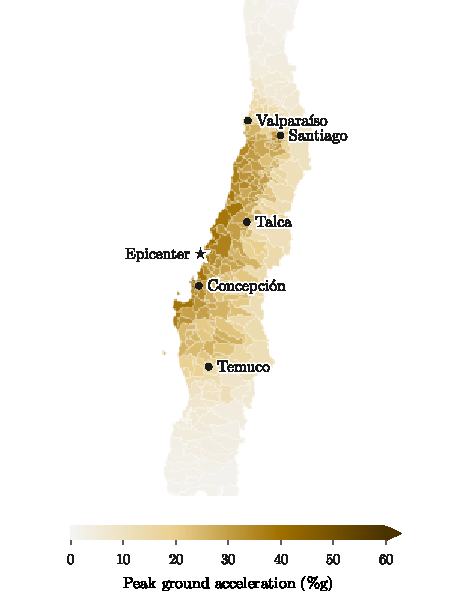
\includegraphics[height=0.7\textheight]{figuras/mapa_pga.pdf}
\notatabla{Peak ground acceleration of the 27-F earthquake, in percent of
gravity, at the centroid of each municipality. Affected municipalities in
the main specification are those of the six regions with destructive
shaking; the map shows how shaking varied within and across them.
\emph{Source:} USGS ShakeMap of the event.}
\end{frame}

\begin{frame}[label=tabdesc]
\titulotabla{Table A1---Descriptive Statistics}{}{datos}
\setlength{\anchotabla}{0.8\textwidth}\setlength{\anchonota}{\anchotabla}
\centering
{\scriptsize\renewcommand{\arraystretch}{0.76}\begin{tabular*}{\anchotabla}{@{\extracolsep{\fill}}l*{4}{c}@{}}
\toprule
 & \multicolumn{2}{c}{All} & \multicolumn{2}{c}{Mean by sex} \\
\cmidrule(lr){2-3} \cmidrule(lr){4-5}
 & (1) & (2) & (3) & (4) \\
 & Mean & SD & Girls & Boys \\
\midrule
\multicolumn{5}{@{}l}{\emph{Panel A. Adolescent, 2024}} \\
PHQ-4 score (0--12) & 4.32 & 2.68 & 4.89 & 3.78 \\
PHQ-4 of 6 or more (share) & 0.27 & 0.44 & 0.34 & 0.19 \\
Age at interview (years) & 16.76 & 1.05 & 16.76 & 16.75 \\
Age at the earthquake (months) & 27.06 & 12.64 & 27.06 & 27.06 \\
Affected municipality (share) & 0.78 & 0.42 & 0.78 & 0.78 \\
\addlinespace[3pt]
\multicolumn{5}{@{}l}{\emph{Panel B. Birth and household, 2010}} \\
Birth weight (kg) & 3.39 & 0.50 & 3.34 & 3.44 \\
Gestation (weeks) & 38.64 & 2.01 & 38.69 & 38.59 \\
Mother's age (years) & 29.52 & 7.11 & 29.60 & 29.44 \\
Mother's education (years) & 10.31 & 3.18 & 10.28 & 10.34 \\
Household size & 4.93 & 1.68 & 4.92 & 4.93 \\
Rural (share) & 0.09 & 0.29 & 0.09 & 0.09 \\
\addlinespace[3pt]
\multicolumn{5}{@{}l}{\emph{Panel C. After the earthquake, 2012}} \\
Breastfed on 27-F (share) & 0.24 & 0.43 & 0.24 & 0.24 \\
Mother reported stress (share) & 0.14 & 0.34 & 0.14 & 0.13 \\
\midrule
Adolescents & 10,003 &  & 4,962 & 5,041 \\
\bottomrule
\end{tabular*}
\par}
\notatabla{Children of the 2010 baseline (15,175) interviewed in 2024 (10,003)
with a PHQ-4 score (9,996); ELPI sampling weights. Panel C was reported in 2012;
breastfed means still breastfed on 27-F.}
\end{frame}

\begin{frame}[label=tabbal]
\titulotabla{Table A2---Balance on Characteristics Fixed Before the
Earthquake}{}{spec}
\setlength{\anchotabla}{0.9\textwidth}\setlength{\anchonota}{\anchotabla}
\centering
{\fontsize{7.5}{9}\selectfont\renewcommand{\arraystretch}{0.9}\begin{tabular*}{\anchotabla}{@{\extracolsep{\fill}}l*{5}{c}@{}}
\toprule
 & \multicolumn{3}{c}{At birth (SD)} & \multicolumn{2}{c}{Mother, 2010 (years)} \\
\cmidrule(lr){2-4} \cmidrule(lr){5-6}
 & (1) & (2) & (3) & (4) & (5) \\
 & Weight & Length & Gestation & Education & Age \\
\midrule
6--11 months $\times$ Affected & 0.193 & 0.037 & 0.109 & $-$0.566 & $-$0.121 \\
 & (0.118) & (0.096) & (0.111) & (0.333) & (0.775) \\
\addlinespace[2pt]
1 year $\times$ Affected & 0.105 & 0.031 & 0.096 & $-$0.481 & $-$0.140 \\
 & (0.103) & (0.100) & (0.086) & (0.264) & (0.695) \\
\addlinespace[2pt]
3--4 years $\times$ Affected & 0.245 & 0.172 & 0.182 & $-$0.350 & 0.457 \\
 & (0.083) & (0.099) & (0.075) & (0.300) & (0.603) \\
\midrule
Observations & 4,530 & 4,526 & 4,819 & 4,883 & 4,921 \\
Municipality FE & Yes & Yes & Yes & Yes & Yes \\
Birth-cohort FE & Yes & Yes & Yes & Yes & Yes \\
Age-group FE & Yes & Yes & Yes & Yes & Yes \\
Controls & No & No & No & No & No \\
\bottomrule
\end{tabular*}
\par}
\notatabla{Girls. Each column regresses a characteristic fixed before the
earthquake on ages 6--17 months $\times$ affected, with municipality, birth-year, and
six-month age-group fixed effects and no controls; the joint test is of a flat profile
across the seven six-month age groups. Birth weight, length, and gestation are
standardized; the mother's education and age were reported in 2010.
Among the 4,190 girls with birth records, the PHQ-4 coefficient for those exposed at 6--17 months, relative to all other ages, is 0.188 (0.079) without and 0.188 (0.079) with the three birth outcomes as controls.
\errores}
\end{frame}

\begin{frame}[label=tabatr]
\titulotabla{Table A3---Attrition between 2010 and 2024}{}{spec}
\setlength{\anchotabla}{0.9\textwidth}\setlength{\anchonota}{\anchotabla}
\centering
{\fontsize{7.5}{9}\selectfont\renewcommand{\arraystretch}{0.9}\begin{tabular*}{\anchotabla}{@{\extracolsep{\fill}}l*{5}{c}@{}}
\toprule
 & \multicolumn{3}{c}{Interviewed in 2024} & \multicolumn{2}{c}{Birth weight, girls (SD)} \\
\cmidrule(lr){2-4} \cmidrule(lr){5-6}
 & (1) & (2) & (3) & (4) & (5) \\
 & Girls & Boys & All & \shortstack{2010\\baseline} & \shortstack{Interviewed\\in 2024} \\
\midrule
6--17 months $\times$ Affected & $-$0.039 & $-$0.012 & $-$0.027 & 0.019 & 0.004 \\
 & (0.029) & (0.029) & (0.020) & (0.065) & (0.079) \\
\midrule
Flat profile, joint test $p$-value & 0.757 & 0.562 & 0.522 & 0.649 & 0.500 \\
Mean of dependent variable & 0.67 & 0.67 & 0.67 &  &  \\
Observations & 6,990 & 7,171 & 14,161 & 6,409 & 4,300 \\
Region FE & Yes & Yes & Yes & Yes & Yes \\
Birth-year FE & Yes & Yes & Yes & Yes & Yes \\
Six-month age-group FE & Yes & Yes & Yes & Yes & Yes \\
\bottomrule
\end{tabular*}
\par}
\notatabla{Children with the 2010 developmental assessment, which gives age in
months (14,161 of 15,175). Columns 1--3 equal one if interviewed in 2024; columns 4--5,
standardized birth weight of all girls assessed in 2010 and of those interviewed in 2024.
Age at the earthquake is the age at the 2010 assessment minus the months from 27-F to the
region's median assessment month, for stayers and leavers alike. Joint test as in
Table A2. The 2010 files do not identify the municipality, so region fixed effects, no
weights, and robust standard errors.}
\end{frame}

\begin{frame}[label=figphq]
\titulotabla{Figure A2---Distribution of the PHQ-4 Score}{}{sm}
\setlength{\anchonota}{\textwidth}
\centering
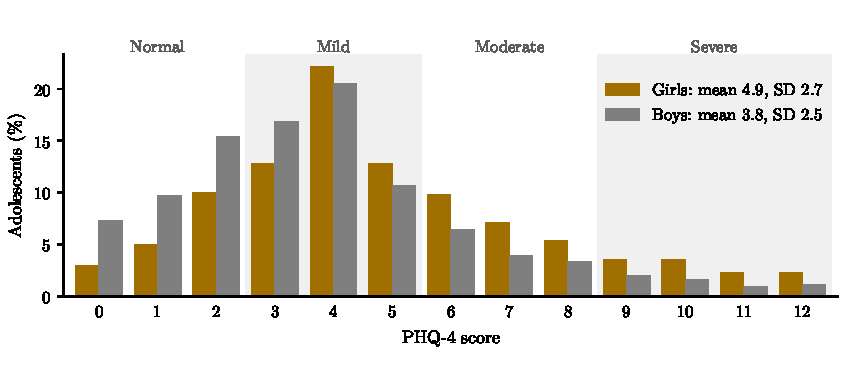
\includegraphics[width=\textwidth]{figuras/phq4_hist.pdf}
\notatabla{PHQ-4 score in 2024, weighted with ELPI sampling weights. The score
adds four items scored 0 to 3; Kroenke et al.\ (2009) classify 0--2 as
normal, 3--5 as mild, 6--8 as moderate, and 9--12 as severe.}
\end{frame}

\begin{frame}[label=figniv]
\titulotabla{Figure A3---PHQ-4 by Age at the Earthquake and Zone}{}{sm}
\setlength{\anchonota}{0.92\textwidth}
\centering
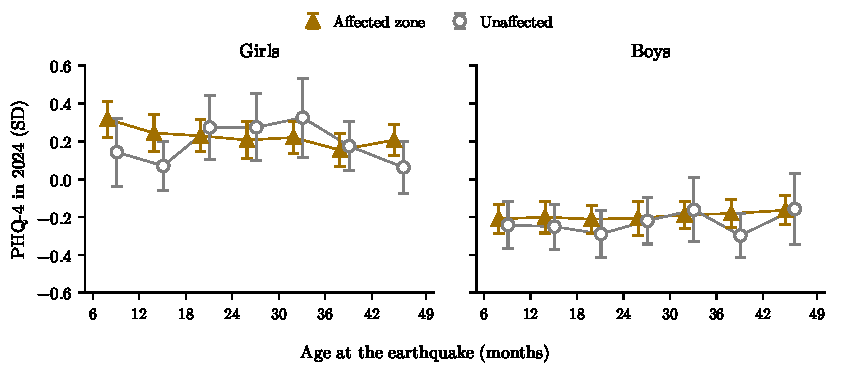
\includegraphics[width=0.92\textwidth]{figuras/niveles.pdf}
\notatabla{Weighted mean of the standardized PHQ-4 in 2024 by six-month age group and
zone; 95\% CI clustered by municipality of selection. Among girls, the affected zone is
nearly flat except at 6--11 months; much of the profile comes from the unaffected zone,
where girls exposed at 6--17 months score low and those exposed at 18--35 months score
high. Relative to ages 36--49 months only, the gap at 6--17 months is 0.10 SD (SE 0.09).}
\end{frame}

\begin{frame}[label=tabphq]
\titulotabla{Table A4---Effect on Mental Health by Age at the Earthquake}{}{sm}
\setlength{\anchotabla}{0.9\textwidth}\setlength{\anchonota}{\anchotabla}
\centering
{\fontsize{6.6}{7.9}\selectfont\renewcommand{\arraystretch}{0.72}\begin{tabular*}{\anchotabla}{@{\extracolsep{\fill}}l*{3}{c}@{}}
\toprule
 & \multicolumn{3}{c}{PHQ-4 (SD)} \\
\cmidrule(lr){2-4}
 & (1) & (2) & (3) \\
 & All & Girls & Boys \\
\midrule
6--11 months & 0.069 & 0.161 & $-$0.014 \\
 & (0.049) & (0.083) & (0.071) \\
12--17 months & 0.075 & 0.143 & 0.015 \\
 & (0.057) & (0.079) & (0.073) \\
18--23 months & $-$0.033 & $-$0.090 & 0.032 \\
 & (0.063) & (0.088) & (0.084) \\
24--29 months & $-$0.055 & $-$0.131 & $-$0.014 \\
 & (0.057) & (0.073) & (0.071) \\
30--35 months & $-$0.103 & $-$0.151 & $-$0.049 \\
 & (0.058) & (0.086) & (0.086) \\
36--41 months & 0.011 & $-$0.044 & 0.070 \\
 & (0.049) & (0.073) & (0.065) \\
42--49 months & 0.036 & 0.113 & $-$0.040 \\
 & (0.054) & (0.074) & (0.092) \\
\midrule
Flat profile, joint test $p$-value & 0.290 & 0.029 & 0.905 \\
Observations & 9,996 & 4,961 & 5,035 \\
Municipality FE & Yes & Yes & Yes \\
Birth-year FE & Yes & Yes & Yes \\
Six-month age-group FE & Yes & Yes & Yes \\
Controls & Yes & Yes & Yes \\
\bottomrule
\end{tabular*}
\par}
\notatabla{Affected minus unaffected municipalities in the standardized PHQ-4 in each
six-month age group, normalized to average zero; the joint test is of equal effects at all
ages. Controls and weights as in Table A5. For girls, the joint test gives $p = 0.03$ with
month-of-birth fixed effects and $p = 0.04$ with peak ground acceleration instead of the
zone. \errores}
\end{frame}

\begin{frame}[label=tabsum]
\titulotabla{Table A5---The First 18 Months Relative to All Other Ages}{}{sm}
\setlength{\anchotabla}{\textwidth}\setlength{\anchonota}{\anchotabla}
\centering
{\fontsize{7.5}{9}\selectfont\renewcommand{\arraystretch}{0.9}\begin{tabular*}{\anchotabla}{@{\extracolsep{\fill}}l*{5}{c}@{}}
\toprule
 & \multicolumn{5}{c}{PHQ-4 (SD)} \\
\cmidrule(lr){2-6}
 & (1) & (2) & (3) & (4) & (5) \\
 & All & Girls & Boys & Girls & Girls \\
\midrule
\multicolumn{6}{@{}l}{\emph{Panel A. Relative to all other ages}} \\
6--11 months $\times$ Affected & 0.077 & 0.180 & $-$0.016 & 0.190 & 0.066 \\
 & (0.057) & (0.097) & (0.083) & (0.097) & (0.030) \\
\addlinespace[3pt]
\multicolumn{6}{@{}l}{\emph{Panel B. Relative to ages 2--3}} \\
6--11 months $\times$ Affected & 0.147 & 0.300 & 0.016 & 0.310 & 0.096 \\
 & (0.069) & (0.100) & (0.098) & (0.101) & (0.029) \\
\addlinespace[2pt]
1--2 years $\times$ Affected & 0.102 & 0.171 & 0.052 & 0.178 & 0.054 \\
 & (0.070) & (0.098) & (0.085) & (0.099) & (0.031) \\
\addlinespace[2pt]
3--4 years $\times$ Affected & 0.103 & 0.182 & 0.042 & 0.177 & 0.034 \\
 & (0.060) & (0.086) & (0.086) & (0.089) & (0.028) \\
\midrule
Observations & 9,996 & 4,961 & 5,035 & 4,961 & 4,961 \\
Municipality FE & Yes & Yes & Yes & Yes & Yes \\
Birth-year FE & Yes & Yes & Yes & No & Yes \\
Age-group FE & Yes & Yes & Yes & No & Yes \\
Month-of-birth FE & No & No & No & Yes & No \\
Exposure & Zone & Zone & Zone & Zone & PGA \\
Controls & Yes & Yes & Yes & Yes & Yes \\
Wild bootstrap $p$-value, panel A & 0.185 & 0.075 & 0.866 & 0.068 & 0.043 \\
\bottomrule
\end{tabular*}
\par}
\notatabla{Affected minus unaffected municipalities in the standardized PHQ-4 at ages 6--17
months relative to all other ages, a comparison chosen after inspecting Table A4. Controls
are a linear trend in month of birth, sex, the mother's age and education, household size,
rural residence (2010), the mother's number of children, and family history of mental
illness (2012). Column 4 uses month-of-birth fixed effects; column 5, peak ground
acceleration per 10 points of percent of $g$ (28 more in the average affected municipality).
Wild bootstrap with 9,999 Rademacher draws under the null. For girls, randomization
inference over the 5,005 ways of choosing six of the 15 regions as affected gives
$p = 0.06$; with standard errors clustered by region, $p = 0.02$. Girls minus boys, 0.205
(0.099), from a model with every term interacted with sex. ELPI weights. \errores}
\end{frame}

\begin{frame}[label=tabgir]
\titulotabla{Table A6---Other Outcomes, Girls}{}{sm}
\setlength{\anchotabla}{1.1\textwidth}\setlength{\anchonota}{\textwidth}
\centering
{\scriptsize\renewcommand{\arraystretch}{0.85}\resizebox{\textwidth}{!}{\begin{tabular*}{\anchotabla}{@{\extracolsep{\fill}}l*{5}{c}@{}}
\toprule
 & \multicolumn{3}{c}{Adolescent report (SD)} & \multicolumn{2}{c}{Caregiver report, CBCL (SD)} \\
\cmidrule(lr){2-4} \cmidrule(lr){5-6}
 & (1) & (2) & (3) & (4) & (5) \\
 & PHQ-4 & Substance use & Victimization & Internalizing & Externalizing \\
\midrule
6--17 months $\times$ Affected & 0.206 & 0.077 & 0.006 & 0.085 & 0.077 \\
 & (0.075) & (0.074) & (0.076) & (0.082) & (0.073) \\
\midrule
Flat profile, joint test $p$-value & 0.029 & 0.548 & 0.007 & 0.638 & 0.337 \\
Observations & 4,961 & 4,961 & 4,539 & 4,748 & 4,748 \\
Municipality FE & Yes & Yes & Yes & Yes & Yes \\
Birth-year FE & Yes & Yes & Yes & Yes & Yes \\
Six-month age-group FE & Yes & Yes & Yes & Yes & Yes \\
Controls & Yes & Yes & Yes & Yes & Yes \\
\bottomrule
\end{tabular*}
}\par}
\notatabla{Girls. Each column is a separate regression with the specification of
Table A5. The adolescent reports the PHQ-4, substance use (any alcohol, tobacco,
cannabis, or other drug in the last 12 months), and peer victimization; the caregiver
reports internalizing and externalizing problems (CBCL). All measured in 2024 and
standardized; higher is worse. Boys in Table A7. \errores}
\end{frame}

\begin{frame}[label=tabboy]
\titulotabla{Table A7---Other Outcomes, Boys}{}{sm}
\setlength{\anchotabla}{1.1\textwidth}\setlength{\anchonota}{\textwidth}
\centering
{\scriptsize\renewcommand{\arraystretch}{0.85}\resizebox{\textwidth}{!}{\begin{tabular*}{\anchotabla}{@{\extracolsep{\fill}}l*{5}{c}@{}}
\toprule
 & \multicolumn{3}{c}{Adolescent report (SD)} & \multicolumn{2}{c}{Caregiver report, CBCL (SD)} \\
\cmidrule(lr){2-4} \cmidrule(lr){5-6}
 & (1) & (2) & (3) & (4) & (5) \\
 & PHQ-4 & Substance use & Victimization & Internalizing & Externalizing \\
\midrule
\multicolumn{6}{@{}l}{\emph{Panel A. Relative to all other ages}} \\
6--11 months $\times$ Affected & $-$0.016 & 0.203 & 0.066 & 0.029 & 0.082 \\
 & (0.083) & (0.085) & (0.087) & (0.086) & (0.081) \\
\addlinespace[3pt]
\multicolumn{6}{@{}l}{\emph{Panel B. Relative to ages 2--3}} \\
6--11 months $\times$ Affected & 0.016 & 0.172 & 0.136 & 0.012 & 0.144 \\
 & (0.098) & (0.104) & (0.106) & (0.100) & (0.079) \\
\addlinespace[2pt]
1--2 years $\times$ Affected & 0.052 & $-$0.064 & 0.112 & $-$0.063 & 0.053 \\
 & (0.085) & (0.089) & (0.086) & (0.099) & (0.092) \\
\addlinespace[2pt]
3--4 years $\times$ Affected & 0.042 & $-$0.031 & 0.098 & 0.010 & 0.126 \\
 & (0.086) & (0.079) & (0.094) & (0.099) & (0.090) \\
\midrule
Observations & 5,035 & 5,034 & 4,637 & 4,804 & 4,804 \\
Municipality FE & Yes & Yes & Yes & Yes & Yes \\
Birth-year FE & Yes & Yes & Yes & Yes & Yes \\
Age-group FE & Yes & Yes & Yes & Yes & Yes \\
Controls & Yes & Yes & Yes & Yes & Yes \\
\bottomrule
\end{tabular*}
}\par}
\notatabla{Boys. Outcomes and specification as in Table A6. \errores}
\end{frame}

\begin{frame}[label=tabola]
\titulotabla{Table A8---Mental Health in Three Rounds}{}{olas}
\setlength{\anchotabla}{\textwidth}\setlength{\anchonota}{\anchotabla}
\centering
{\fontsize{7}{8.4}\selectfont\renewcommand{\arraystretch}{0.8}\begin{tabular*}{\anchotabla}{@{\extracolsep{\fill}}l*{5}{c}@{}}
\toprule
 & \multicolumn{3}{c}{Caregiver, CBCL internalizing (SD)} & \multicolumn{2}{c}{Own report (SD)} \\
\cmidrule(lr){2-4} \cmidrule(lr){5-6}
 & (1) & (2) & (3) & (4) & (5) \\
 & \shortstack{2012\\ages 2--6} & \shortstack{2017\\ages 8--12} & \shortstack{2024\\ages 14--18} & \shortstack{2017\\ages 8--12} & \shortstack{2024\\ages 14--18} \\
\midrule
\multicolumn{6}{@{}l}{\emph{Panel A. Girls}} \\
6--17 months $\times$ Affected & 0.000 & 0.039 & 0.081 & 0.150 & 0.206 \\
 & (0.089) & (0.097) & (0.078) & (0.123) & (0.075) \\
Flat profile, joint test $p$-value & 0.215 & 0.944 & 0.833 & 0.479 & 0.029 \\
Observations & 4,053 & 3,533 & 4,946 & 3,510 & 4,961 \\
\addlinespace[3pt]
\multicolumn{6}{@{}l}{\emph{Panel B. Boys}} \\
6--17 months $\times$ Affected & $-$0.003 & 0.059 & 0.064 & 0.098 & 0.001 \\
 & (0.073) & (0.116) & (0.069) & (0.068) & (0.064) \\
Flat profile, joint test $p$-value & 0.987 & 0.211 & 0.748 & 0.881 & 0.905 \\
Observations & 4,087 & 3,650 & 5,024 & 3,603 & 5,035 \\
\midrule
Municipality FE & Yes & Yes & Yes & Yes & Yes \\
Birth-year FE & Yes & Yes & Yes & Yes & Yes \\
Six-month age-group FE & Yes & Yes & Yes & Yes & Yes \\
Controls & Yes & Yes & Yes & Yes & Yes \\
\bottomrule
\end{tabular*}
\par}
\notatabla{The adolescents interviewed in 2024, in each round in which they have the
measure; specification of Table A5, with 2024 weights. Caregiver: CBCL
internalizing scale, standardized. Own report: in 2017, the mean of three standardized
items (low self-esteem, not feeling happy, feeling lonely in class); in 2024, the PHQ-4.
Higher is worse. \errores}
\end{frame}

\begin{frame}[label=figola]
\titulotabla{Figure A4---The Age Profile in Three Rounds}{}{olas}
\setlength{\anchonota}{0.88\textwidth}
\centering
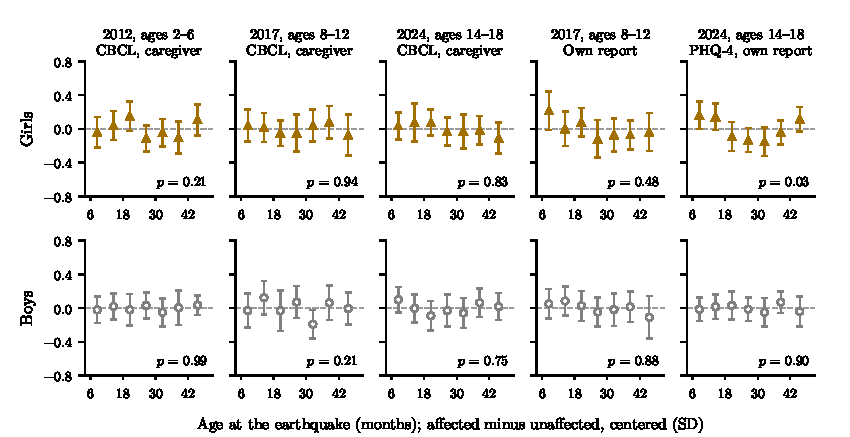
\includegraphics[width=0.88\textwidth]{figuras/olas_perfiles.pdf}
\notatabla{For each measure of Table A8, affected minus unaffected in each six-month age
group, normalized to average zero; 95\% CI. $p$, joint test of a flat profile.}
\end{frame}

\begin{frame}[label=tabent]
\titulotabla{Table A9---The Socioeconomic and Family Environment}{}{entorno}
\setlength{\anchotabla}{1.1\textwidth}\setlength{\anchonota}{\textwidth}
\centering
{\scriptsize\renewcommand{\arraystretch}{0.82}\resizebox{\textwidth}{!}{\begin{tabular*}{\anchotabla}{@{\extracolsep{\fill}}l*{6}{c}@{}}
\toprule
 & \multicolumn{3}{c}{Mechanisms in Gillmore (2026), SD} & \multicolumn{3}{c}{Other household conditions, SD} \\
\cmidrule(lr){2-4} \cmidrule(lr){5-7}
 & (1) & (2) & (3) & (4) & (5) & (6) \\
 & \shortstack{Lower\\income} & \shortstack{Mother not\\employed} & \shortstack{Damaged\\housing} & \shortstack{Conflict\\at home} & \shortstack{Overcrowded\\housing} & \shortstack{Precarious\\housing} \\
\midrule
6--17 months $\times$ Affected & $-$0.013 & $-$0.188 & $-$0.005 & $-$0.152 & 0.000 & 0.051 \\
 & (0.064) & (0.065) & (0.049) & (0.073) & (0.065) & (0.061) \\
\midrule
Flat profile, joint test $p$-value & 0.880 & 0.088 & 0.944 & 0.027 & 0.366 & 0.615 \\
Observations & 4,478 & 4,925 & 4,423 & 4,701 & 4,961 & 4,960 \\
Municipality FE & Yes & Yes & Yes & Yes & Yes & Yes \\
Birth-year FE & Yes & Yes & Yes & Yes & Yes & Yes \\
Six-month age-group FE & Yes & Yes & Yes & Yes & Yes & Yes \\
Controls & Yes & Yes & Yes & Yes & Yes & Yes \\
\bottomrule
\end{tabular*}
}\par}
\notatabla{Girls. Each column is a standardized index of the household
environment; higher is worse. Measured in 2010, one to nine months after the
earthquake, except housing damage, reported in 2012. Lower income, per
capita; damaged housing, destroyed or with major damage; conflict at home,
the mother shouting, being hostile, or hitting during the visit; overcrowded
housing, persons per bedroom; precarious housing, an emergency shack or a
lent or shared dwelling. Specification of Table A5. \errores}
\end{frame}

\begin{frame}[label=tablac]
\titulotabla{Table A10---Breastfeeding and the Effect in the First 18 Months}{}{diada}
\setlength{\anchotabla}{0.9\textwidth}\setlength{\anchonota}{\anchotabla}
\centering
{\scriptsize\renewcommand{\arraystretch}{0.76}\begin{tabular*}{\anchotabla}{@{\extracolsep{\fill}}l*{3}{c}@{}}
\toprule
 & \multicolumn{3}{c}{PHQ-4 (SD)} \\
\cmidrule(lr){2-4}
 & (1) & (2) & (3) \\
 & Girls & Girls & Boys \\
\midrule
6--17 months $\times$ Affected $\times$ breastfed & 0.318 & 0.295 & 0.082 \\
 & (0.110) & (0.110) & (0.091) \\
\addlinespace[2pt]
6--17 months $\times$ Affected $\times$ not breastfed & 0.091 & 0.081 & $-$0.045 \\
 & (0.129) & (0.131) & (0.081) \\
\addlinespace[2pt]
Difference, breastfed $-$ not breastfed & 0.227 & 0.214 & 0.127 \\
 & (0.167) & (0.167) & (0.112) \\
\midrule
Wild bootstrap $p$-value, difference & 0.200 & 0.225 & 0.285 \\
Breastfed, share at 6--17 months & 0.53 & 0.54 & 0.51 \\
Observations & 4,409 & 4,338 & 4,465 \\
Municipality FE & Yes & Yes & Yes \\
Birth-year FE & Yes & Yes & Yes \\
Six-month age-group FE & Yes & Yes & Yes \\
Six-month age group $\times$ breastfed FE & Yes & Yes & Yes \\
Controls & Yes & Yes & Yes \\
Mother's education and employment $\times$ breastfed and $\times$ affected & No & Yes & No \\
\bottomrule
\end{tabular*}
\par}
\notatabla{Difference between affected and unaffected municipalities in the
standardized PHQ-4 for those aged 6--17 months, relative to all other ages,
separately for those still breastfed on 27-F (2012 report) and those who were
not. Column 2 lets breastfeeding and the affected zone vary with the mother's
education and employment (2010). Controls, weights, and wild bootstrap as in
Table A5. \errores}
\end{frame}

\begin{frame}[label=figlac]
\titulotabla{Figure A5---Breastfeeding and the Effect of the Earthquake by
Age}{}{diada}
\setlength{\anchonota}{0.9\textwidth}
\centering
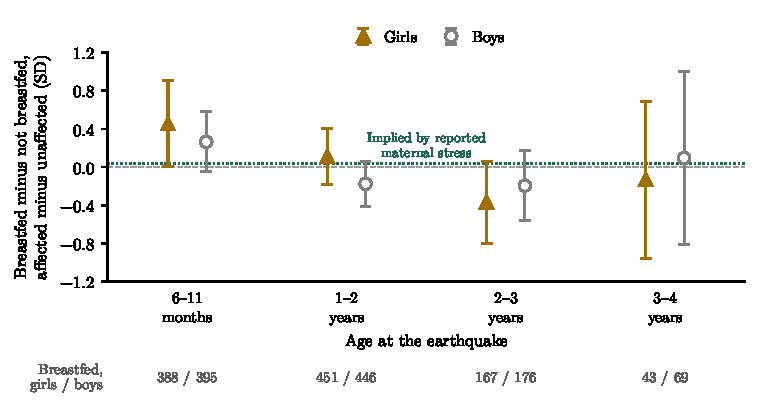
\includegraphics[height=0.62\textheight]{figuras/triple_did.pdf}
\notatabla{For each age at the earthquake, the difference between affected and
unaffected municipalities among those breastfed on 27-F minus the same
difference among those who were not, with fixed effects for age group
$\times$ breastfed, municipality, and birth year, and the controls of Table A5.
The dotted line is the value implied by maternal stress reported in 2012
(0.29 $\times$ 0.13). 95\% CI.}
\end{frame}

\begin{frame}[label=tabdia]
\titulotabla{Table A11---Maternal Stress, Breastfeeding, and Daughters'
Mental Health}{}{diada}
\setlength{\anchotabla}{\textwidth}\setlength{\anchonota}{\textwidth}
\centering
{\scriptsize\renewcommand{\arraystretch}{0.84}\begin{tabular*}{\anchotabla}{@{\extracolsep{\fill}}l*{3}{c}@{}}
\toprule
 & \multicolumn{3}{c}{Daughters' PHQ-4 (SD)} \\
\cmidrule(lr){2-4}
 & (1) & (2) & (3) \\
 & Baseline & \shortstack{Mother's\\SES} & \shortstack{Mother's SES\\and 6--17 months} \\
\midrule
Maternal stress $\times$ not breastfed & $-$0.026 & $-$0.006 & $-$0.024 \\
 & (0.056) & (0.064) & (0.069) \\
\addlinespace[2pt]
Maternal stress $\times$ breastfed & 0.294 & 0.284 & 0.213 \\
 & (0.088) & (0.096) & (0.119) \\
\addlinespace[2pt]
Difference, breastfed $-$ not breastfed & 0.320 & 0.290 & 0.237 \\
 & (0.108) & (0.101) & (0.109) \\
\midrule
Observations & 4,409 & 4,377 & 4,377 \\
Municipality FE & Yes & Yes & Yes \\
Birth-year FE & Yes & Yes & Yes \\
Six-month age-group FE & Yes & Yes & Yes \\
Six-month age group $\times$ breastfed FE & Yes & Yes & Yes \\
Controls & Yes & Yes & Yes \\
Stress and breastfed $\times$ mother's education and employment & No & Yes & Yes \\
Stress $\times$ 6--17 months & No & No & Yes \\
\bottomrule
\end{tabular*}
\par}
\notatabla{Girls, all ages. Maternal stress equals one if the mother reported stress,
distress, or anxiety after the earthquake (2012); breastfed equals one if
the child was still breastfed on 27-F (2012 report). Column 2 lets stress and
breastfeeding vary with the mother's education and employment (2010); column 3
also lets stress vary at 6--17 months. Controls and weights as in Table A5.
\errores}
\end{frame}

\begin{frame}[label=tabmed]
\titulotabla{Table A12---Maternal Stress and Breastfeeding by Age at the
Earthquake}{}{diada}
\setlength{\anchotabla}{0.7\textwidth}\setlength{\anchonota}{\anchotabla}
\centering
{\fontsize{7}{8.4}\selectfont\renewcommand{\arraystretch}{0.78}\begin{tabular*}{\anchotabla}{@{\extracolsep{\fill}}l*{3}{c}@{}}
\toprule
 & \multicolumn{2}{c}{Mothers with stress (\%)} & \multicolumn{1}{c}{Breastfed (\%)} \\
\cmidrule(lr){2-3} \cmidrule(lr){4-4}
 & (1) & (2) & (3) \\
 & Affected & Unaffected & On 27-F \\
\midrule
6--11 months & 15.0 & 3.8 & 61.8 \\
 & (1.2) & (1.1) & (1.4) \\
12--17 months & 16.1 & 3.2 & 42.6 \\
 & (1.2) & (1.0) & (1.4) \\
18--23 months & 15.0 & 4.0 & 30.3 \\
 & (1.2) & (1.2) & (1.3) \\
24--29 months & 17.5 & 4.1 & 15.6 \\
 & (1.2) & (1.2) & (1.0) \\
30--35 months & 18.1 & 3.2 & 12.9 \\
 & (1.3) & (1.0) & (1.0) \\
36--41 months & 19.2 & 2.6 & 5.0 \\
 & (1.3) & (0.9) & (0.6) \\
42--49 months & 16.6 & 3.7 & 3.3 \\
 & (1.1) & (1.0) & (0.5) \\
\midrule
Observations & 6,772 & 2,132 & 8,874 \\
\bottomrule
\end{tabular*}
\par}
\notatabla{Unweighted means, with standard errors in parentheses, by the
child's age at the earthquake, among the adolescents of Table A1 whose
mother answered each question in 2012. Columns 1 and 2 report the share of
mothers who reported stress, distress, or anxiety after the earthquake, in
affected and unaffected municipalities; column 3, the share of children
still breastfed on 27-F.}
\end{frame}

\end{document}
